% Options for packages loaded elsewhere
\PassOptionsToPackage{unicode}{hyperref}
\PassOptionsToPackage{hyphens}{url}
%
\documentclass[
]{article}
\usepackage{lmodern}
\usepackage{amssymb,amsmath}
\usepackage{ifxetex,ifluatex}
\ifnum 0\ifxetex 1\fi\ifluatex 1\fi=0 % if pdftex
  \usepackage[T1]{fontenc}
  \usepackage[utf8]{inputenc}
  \usepackage{textcomp} % provide euro and other symbols
\else % if luatex or xetex
  \usepackage{unicode-math}
  \defaultfontfeatures{Scale=MatchLowercase}
  \defaultfontfeatures[\rmfamily]{Ligatures=TeX,Scale=1}
\fi
% Use upquote if available, for straight quotes in verbatim environments
\IfFileExists{upquote.sty}{\usepackage{upquote}}{}
\IfFileExists{microtype.sty}{% use microtype if available
  \usepackage[]{microtype}
  \UseMicrotypeSet[protrusion]{basicmath} % disable protrusion for tt fonts
}{}
\makeatletter
\@ifundefined{KOMAClassName}{% if non-KOMA class
  \IfFileExists{parskip.sty}{%
    \usepackage{parskip}
  }{% else
    \setlength{\parindent}{0pt}
    \setlength{\parskip}{6pt plus 2pt minus 1pt}}
}{% if KOMA class
  \KOMAoptions{parskip=half}}
\makeatother
\usepackage{xcolor}
\IfFileExists{xurl.sty}{\usepackage{xurl}}{} % add URL line breaks if available
\IfFileExists{bookmark.sty}{\usepackage{bookmark}}{\usepackage{hyperref}}
\hypersetup{
  pdftitle={Supplementary Information},
  hidelinks,
  pdfcreator={LaTeX via pandoc}}
\urlstyle{same} % disable monospaced font for URLs
\usepackage[margin=1in]{geometry}
\usepackage{longtable,booktabs}
% Correct order of tables after \paragraph or \subparagraph
\usepackage{etoolbox}
\makeatletter
\patchcmd\longtable{\par}{\if@noskipsec\mbox{}\fi\par}{}{}
\makeatother
% Allow footnotes in longtable head/foot
\IfFileExists{footnotehyper.sty}{\usepackage{footnotehyper}}{\usepackage{footnote}}
\makesavenoteenv{longtable}
\usepackage{graphicx,grffile}
\makeatletter
\def\maxwidth{\ifdim\Gin@nat@width>\linewidth\linewidth\else\Gin@nat@width\fi}
\def\maxheight{\ifdim\Gin@nat@height>\textheight\textheight\else\Gin@nat@height\fi}
\makeatother
% Scale images if necessary, so that they will not overflow the page
% margins by default, and it is still possible to overwrite the defaults
% using explicit options in \includegraphics[width, height, ...]{}
\setkeys{Gin}{width=\maxwidth,height=\maxheight,keepaspectratio}
% Set default figure placement to htbp
\makeatletter
\def\fps@figure{htbp}
\makeatother
\setlength{\emergencystretch}{3em} % prevent overfull lines
\providecommand{\tightlist}{%
  \setlength{\itemsep}{0pt}\setlength{\parskip}{0pt}}
\setcounter{secnumdepth}{-\maxdimen} % remove section numbering
\usepackage{setspace}
\setstretch{1,5}
\usepackage{lineno}
\usepackage{lscape}
\linenumbers

\title{Supplementary Information}
\date{}

\begin{document}
\maketitle

\hypertarget{supplementary-tables}{%
\section{Supplementary Tables}\label{supplementary-tables}}

\textbf{Table S1}. List of species included in the analyses and their
traits. The species groups were defined using their trait values and
knowledge of species ecology. Temperate species have temperature indices
above 4.25, and boreal species below 4.25. Pioneer species have shade
tolerance below 2.6 and are generally found in disturbed habitats.

\begin{longtable}[]{@{}lllll@{}}
\toprule
Species name & Vernacular name & Group & Shade tolerance & Temperature
index\tabularnewline
\midrule
\endhead
Abies balsamea & Balsam fir & Boreal & 5.0 & 3.16\tabularnewline
Acer pensylvanicum & Striped maple & Temperate & 3.5 &
5.22\tabularnewline
Acer rubrum & Red maple & Temperate & 3.4 & 9.28\tabularnewline
Acer saccharinum & Silver maple & Temperate & 3.6 & 9.97\tabularnewline
Acer saccharum & Sugar maple & Temperate & 4.8 & 6.93\tabularnewline
Acer spicatum & Mountain maple & Temperate & 3.3 & 4.52\tabularnewline
Alnus incana & Speckled alder & Boreal & 1 & 1.22\tabularnewline
Amelanchier sp. & Serviceberry & Temperate & 3.4 & 9.40\tabularnewline
Betula alleghaniensis & Yellow birch & Temperate & 3.2 &
4.49\tabularnewline
Betula papyrifera & White birch & Pioneer & 1.5 & 3.69\tabularnewline
Betula populifolia & Grey birch & Pioneer & 1.5 & 5.58\tabularnewline
Carpinus caroliniana & Blue beech & Temperate & 4.6 &
15.90\tabularnewline
Carya cordiformis & Bitternut hickory & Temperate & 2.1 &
11.06\tabularnewline
Fagus grandifolia & American beech & Temperate & 4.8 &
8.46\tabularnewline
Fraxinus americana & White ash & Temperate & 2.5 & 9.54\tabularnewline
Fraxinus nigra & Black ash & Temperate & 3 & 4.92\tabularnewline
Fraxinus pennsylvanica & Red ash & Temperate & 3.1 &
11.86\tabularnewline
Juglans cinerea & Butternut & Temperate & 1.9 & 8.10\tabularnewline
Larix laricina & Tamarack & Boreal & 1 & 3.92\tabularnewline
Malus sp. & Crab apple & Temperate & 2.2 & 7.96\tabularnewline
Ostrya virginiana & Ironwood & Temperate & 4.6 & 8.91\tabularnewline
Picea glauca & White spruce & Boreal & 4.2 & 3.08\tabularnewline
Picea mariana & Black spruce & Boreal & 4.1 & 1.68\tabularnewline
Picea rubens & Red spruce & Temperate & 4.4 & 4.26\tabularnewline
Pinus banksiana & Jack pine & Boreal & 1.4 & 2.99\tabularnewline
Pinus resinosa & Red pine & Temperate & 1.9 & 5.54\tabularnewline
Pinus strobus & Eastern white pine & Temperate & 3.2 &
6.85\tabularnewline
Populus balsamifera & Balsam poplar & Pioneer & 1.3 &
4.25\tabularnewline
Populus deltoides & Cottonwood & Pioneer & 1.8 & 8.12\tabularnewline
Populus grandidentata & Large tooth aspen & Pioneer & 1.2 &
6.14\tabularnewline
Populus tremuloides & Trembling aspen & Pioneer & 1.2 &
4.22\tabularnewline
Prunus pensylvanica & Pin cherry & Pioneer & 1 & 4.01\tabularnewline
Prunus serotina & Black cherry & Temperate & 2.5 & 4.69\tabularnewline
Prunus virginiana & Chokecherry & Temperate & 2.6 & 7.79\tabularnewline
Quercus alba & White oak & Temperate & 2.9 & 12.95\tabularnewline
Quercus bicolor & Swamp white oak & Temperate & 3 & 9.51\tabularnewline
Quercus macrocarpa & Bur oak & Temperate & 2.7 & 6.72\tabularnewline
Quercus rubra & Red oak & Temperate & 2.8 & 9.67\tabularnewline
Salix sp. & Willow & Pioneer & 1.5 & 13.32\tabularnewline
Sorbus sp. & Mountain-ash & Pioneer & 2.6 & 2.31\tabularnewline
Thuja occidentalis & White cedar & Temperate & 3.5 & 4.30\tabularnewline
Tilia americana & Basswood & Temperate & 4 & 5.34\tabularnewline
Tsuga canadensis & Eastern hemlock & Temperate & 4.8 &
6.87\tabularnewline
Ulmus americana & American elm & Temperate & 3.1 & 10.67\tabularnewline
Ulmus rubra & Red elm & Temperate & 3.3 & 12.37\tabularnewline
Ulmus thomasii & Rock elm & Temperate & 3.2 & 7.80\tabularnewline
\bottomrule
\end{longtable}

\pagebreak

\textbf{Table S2}. 21 original disturbance types and their
reclassification into natural disturbances and harvest, with three
levels of intensity. Sites with tree planting were excluded from the
study.

\begin{longtable}[]{@{}llll@{}}
\toprule
& Original disturbance types & Reclassification & Disturbance
level\tabularnewline
\midrule
\endhead
1 & Improvement cutting & Harvest & Moderate\tabularnewline
2 & Strip cutting & Harvest & Moderate\tabularnewline
3 & Checkerboard~clear-cutting & Harvest & Moderate\tabularnewline
4 & Diameter-limit cutting & Harvest & Moderate\tabularnewline
5 & Selection cutting & Harvest & Moderate\tabularnewline
6 & Partial cutting & Harvest & Moderate\tabularnewline
7 & Diameter-limit cutting with crop tree release & Harvest &
Moderate\tabularnewline
8 & Commercial~thinning & Harvest & Moderate\tabularnewline
9 & Partial cutting with light outbreak & Harvest &
Moderate\tabularnewline
10 & Partial burn & Natural & Moderate\tabularnewline
11 & Light outbreak & Natural & Moderate\tabularnewline
12 & Partial windfall & Natural & Moderate\tabularnewline
13 & Partial ice storm & Natural & Moderate\tabularnewline
14 & Partial decline & Natural & Moderate\tabularnewline
15 & Final strip cutting & Harvest & Major\tabularnewline
16 & Harvesting~with protection of regeneration & Harvest &
Major\tabularnewline
17 & Clearcutting & Harvest & Major\tabularnewline
18 & Total burn & Natural & Major\tabularnewline
19 & Severe outbreak & Natural & Major\tabularnewline
20 & Total windfall & Natural & Major\tabularnewline
21 & Total decline & Natural & Major\tabularnewline
- & Seeding & Plantation & x\tabularnewline
- & Planting & Plantation & x\tabularnewline
- & Planting bare-rooted seedlings & Plantation & x\tabularnewline
- & Container planting & Plantation & x\tabularnewline
\bottomrule
\end{longtable}

\pagebreak

\textbf{Table S3}. List of R packages used for analyses.

\begin{longtable}[]{@{}lll@{}}
\toprule
\begin{minipage}[b]{0.15\columnwidth}\raggedright
Packages\strut
\end{minipage} & \begin{minipage}[b]{0.48\columnwidth}\raggedright
Uses\strut
\end{minipage} & \begin{minipage}[b]{0.29\columnwidth}\raggedright
References\strut
\end{minipage}\tabularnewline
\midrule
\endhead
\begin{minipage}[t]{0.15\columnwidth}\raggedright
adespatial\strut
\end{minipage} & \begin{minipage}[t]{0.48\columnwidth}\raggedright
Forward selection (\texttt{forward.sel}), temporal beta diversity
(\texttt{tbi})\strut
\end{minipage} & \begin{minipage}[t]{0.29\columnwidth}\raggedright
Dray et al. (2018)\strut
\end{minipage}\tabularnewline
\begin{minipage}[t]{0.15\columnwidth}\raggedright
FD\strut
\end{minipage} & \begin{minipage}[t]{0.48\columnwidth}\raggedright
Functional composition (\texttt{functcomp})\strut
\end{minipage} & \begin{minipage}[t]{0.29\columnwidth}\raggedright
Laliberté et al. (2014)\strut
\end{minipage}\tabularnewline
\begin{minipage}[t]{0.15\columnwidth}\raggedright
raster\strut
\end{minipage} & \begin{minipage}[t]{0.48\columnwidth}\raggedright
Manipulation of spatial data\strut
\end{minipage} & \begin{minipage}[t]{0.29\columnwidth}\raggedright
Hijmans (2018)\strut
\end{minipage}\tabularnewline
\begin{minipage}[t]{0.15\columnwidth}\raggedright
sf\strut
\end{minipage} & \begin{minipage}[t]{0.48\columnwidth}\raggedright
Manipulation of spatial data\strut
\end{minipage} & \begin{minipage}[t]{0.29\columnwidth}\raggedright
Pebesma (2018)\strut
\end{minipage}\tabularnewline
\begin{minipage}[t]{0.15\columnwidth}\raggedright
stats\strut
\end{minipage} & \begin{minipage}[t]{0.48\columnwidth}\raggedright
Linear regressions (\texttt{lm})\strut
\end{minipage} & \begin{minipage}[t]{0.29\columnwidth}\raggedright
R Core Team (2018)\strut
\end{minipage}\tabularnewline
\begin{minipage}[t]{0.15\columnwidth}\raggedright
vegan\strut
\end{minipage} & \begin{minipage}[t]{0.48\columnwidth}\raggedright
Variation partitioning (\texttt{varpart})\strut
\end{minipage} & \begin{minipage}[t]{0.29\columnwidth}\raggedright
Oksanen et al. (2019)\strut
\end{minipage}\tabularnewline
\begin{minipage}[t]{0.15\columnwidth}\raggedright
zoo\strut
\end{minipage} & \begin{minipage}[t]{0.48\columnwidth}\raggedright
Rolling average (\texttt{rollmean})\strut
\end{minipage} & \begin{minipage}[t]{0.29\columnwidth}\raggedright
Zeileis \& Grothendieck (2005)\strut
\end{minipage}\tabularnewline
\bottomrule
\end{longtable}

\hypertarget{supplementary-figures}{%
\section{Supplementary Figures}\label{supplementary-figures}}

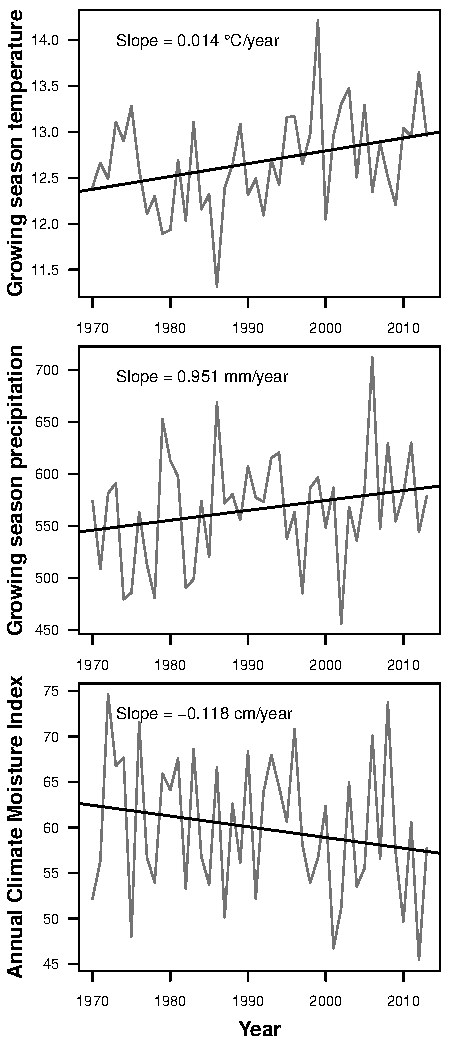
\includegraphics[width=3in,height=\textheight]{ms/figures/figS1_clim_trend.pdf}

\textbf{Figure S1}. Temporal trends in growing season temperatures
(top), total growing season precipitation (middle) and annual climate
moisture index (bottom). Grey lines represent averaged climate values
across the 6281 studied forest plots. Straight black lines show the
fitted least-squared linear regression lines.

\pagebreak

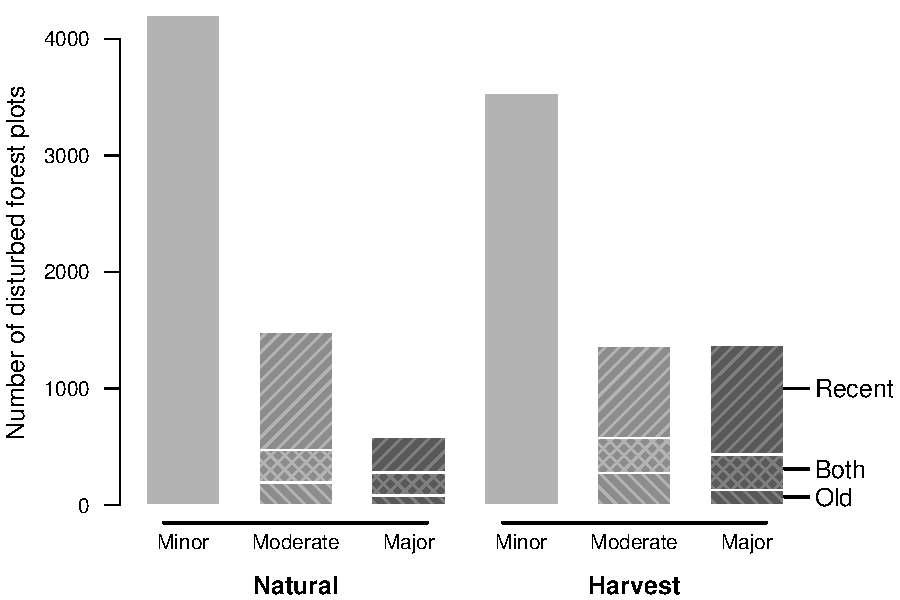
\includegraphics[width=4.5in,height=\textheight]{ms/figures/figS2_disturb.pdf}

\textbf{Figure S2}. Frequency of forest plots by disturbance type
(natural disturbances and harvest), level of intensity (minor, moderate,
major) and timing (old refers to disturbances that occurred before the
study period whereas recent disturbances occurred during the study
period). The three columns in each disturbance type sum to \emph{n} =
6281 forest plots, but many forest plots have been disturbed by more
than one type of disturbance during the study period.

\pagebreak

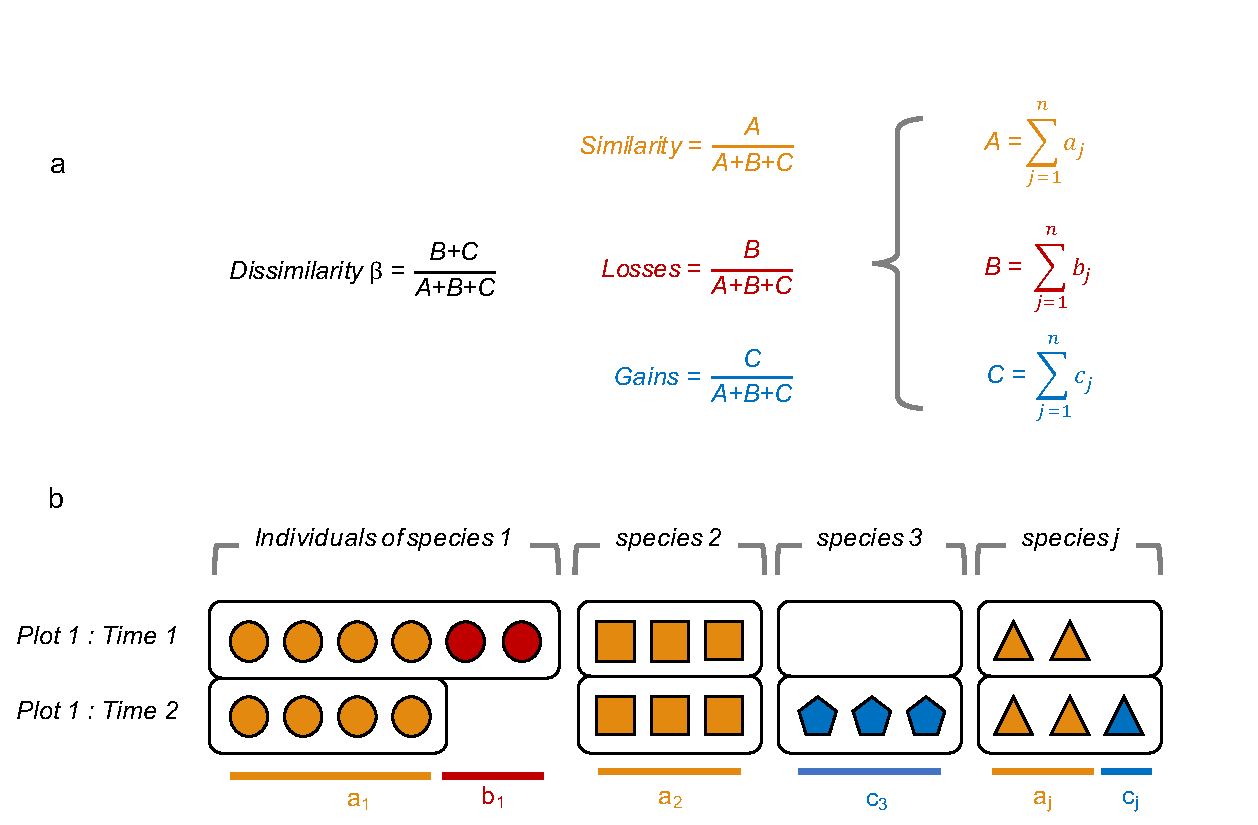
\includegraphics[width=6.6in,height=\textheight]{ms/figures/figS3_beta_calculus.pdf}

\textbf{Figure S3.} Equations to compute the temporal ß diversity index,
as well as its components, using the Ružička coefficient for abundance
data (a) and an example (b) where the tree composition of a single
forest plot is compared between two surveys, \(t_1\) and \(t_2\). In the
example, each of the \(n\) species is represented by a symbol. The
symbols in yellow represent the abundance of a species that is common to
the two survey (component A; note that it can be different individuals
of the same species). The symbols in red represent the abundance of a
species that is lost between \(t_1\) and \(t_2\) (component B). The
symbols in blue represent the abundance of a species that is gained
between \(t_1\) and \(t_2\) (component C). In this example,
\(A = 4 + 3 + 2 = 9\), \(B = 2\), and \(C = 3 + 1 = 4\), therefore
\(\beta = 2+4/(9+2+4) = 0.4\).

\pagebreak

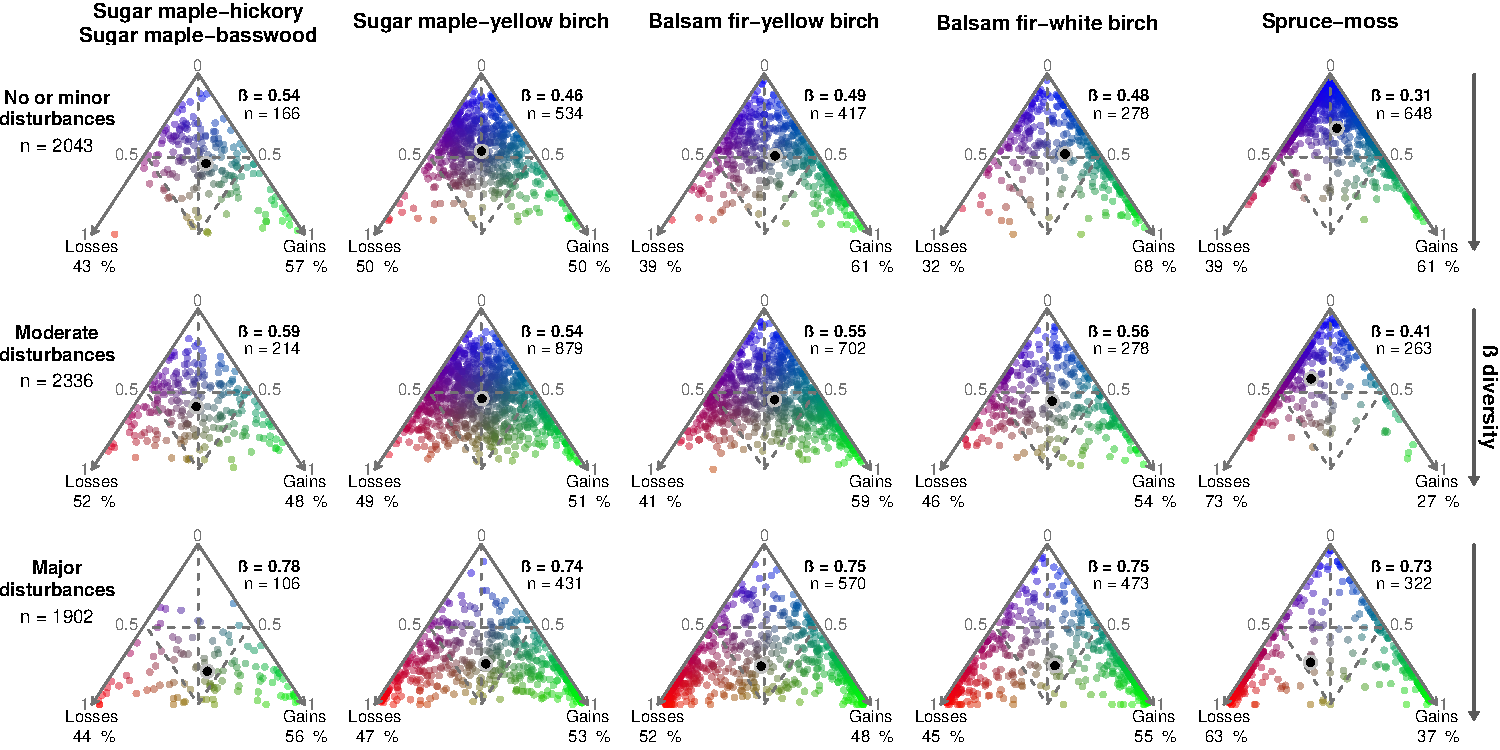
\includegraphics[width=6.6in,height=\textheight]{ms/figures/figS4_ternary.pdf}

\textbf{Figure S4}. Triangular diagrams of gains and losses in tree
abundance by bioclimatic domains and disturbance levels. Each point
represents a forest plot and the large black point represents the
centroid. At the upper tip of the triangle, similarity is high (ß = 0;
blue colors). At the base of the triangle, dissimilarity is high (ß =
1). On the left, forests in red are dominated by losses, while on the
right, forests in green are dominated by gains. The similar
distributions of gain and loss values in the ternary diagrams suggests
that there is no major difference in temporal ß diversity patterns among
domains.

\pagebreak

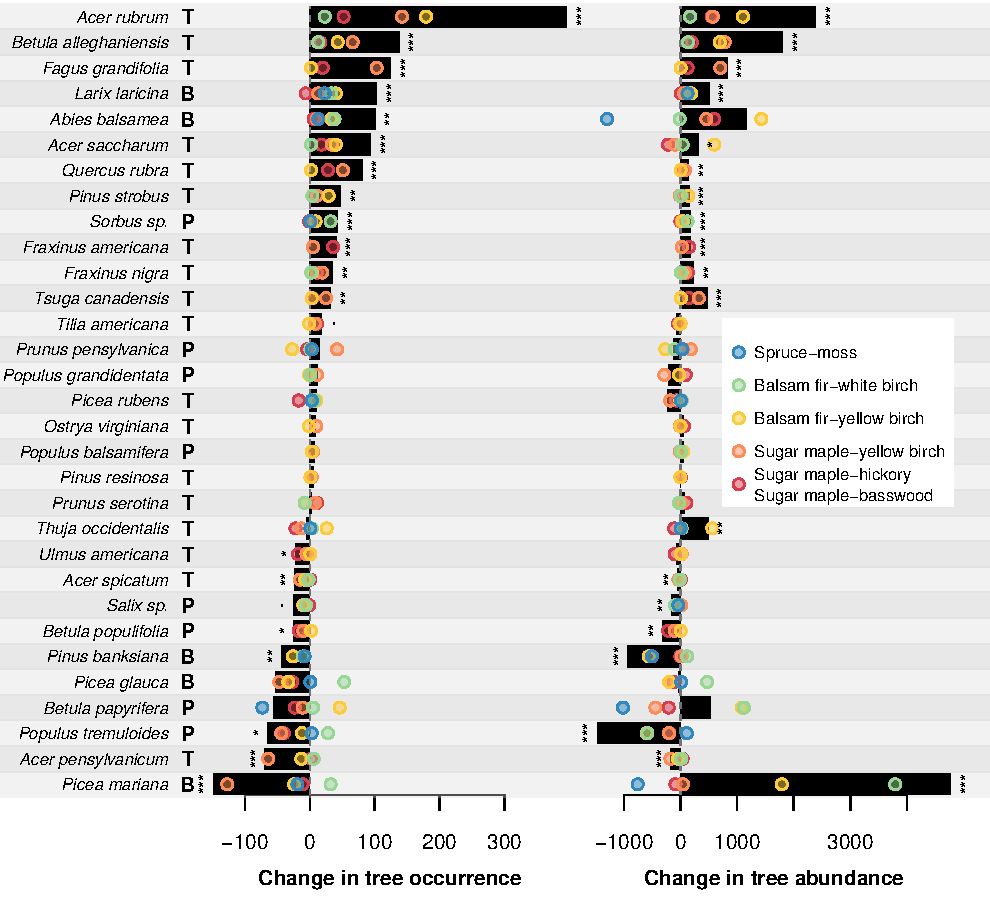
\includegraphics[width=6.6in,height=\textheight]{ms/figures/figS5_spchange.pdf}

\textbf{Figure S5.} Species temporal changes for Québec forests and for
each bioclimatic domain. Changes in species occurrence (left) and
species abundance (right). Only the species occupying more than 20 plots
are shown. The bars represent the mean changes across the study area,
while the colored points represent the mean changes by bioclimatic
domain. Stars represent the levels of the significance of the
\emph{p}-value (* \emph{p} \textless{} 0.05; ** \emph{p} \textless{}
0.01; *** \emph{p} \textless{} 0.001) associated with Wilcoxon
signed-rank tests used to determine whether individual species changes
in occurrence and abundance were significant. An increase in occurrence
indicates that the species has spread regionally, while an increase in
abundance indicates that the species has spread locally and/or
regionally. Letters next to species names correspond to (T)emperate;
(P)ioneer and (B)oreal species.

\pagebreak

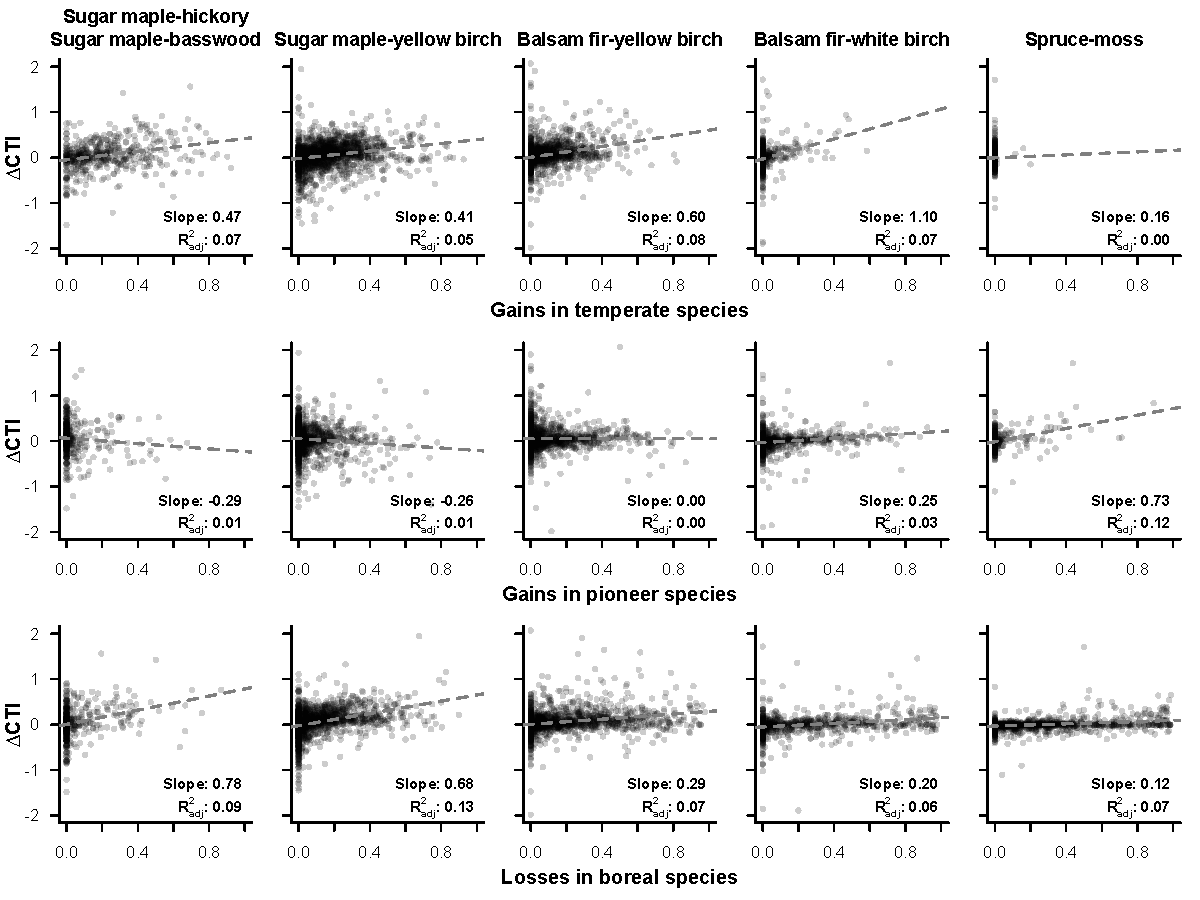
\includegraphics[width=6.6in,height=\textheight]{ms/figures/figS6_CTIvsGains.pdf}

\textbf{Figure S6.} Relations between change in Community Temperature
Index (\(\Delta\)CTI) and gains in temperate (top), gains in pioneer
(middle) and losses in boreal species (bottom). In each panel, the slope
and adjusted \(R^2\) of a linear regression model are shown.

\pagebreak

\hypertarget{references}{%
\section*{References}\label{references}}
\addcontentsline{toc}{section}{References}

\hypertarget{refs}{}
\leavevmode\hypertarget{ref-dray_adespatial_2018}{}%
Dray, S., Bauman, D., Blanchet, G., Borcard, D., Clappe, S., Guenard,
G., Jombart, T., Larocque, G., Legendre, P., Madi, N., \& Wagner, H. H.
(2018). \emph{Adespatial: Multivariate Multiscale Spatial Analysis}.
\url{https://CRAN.R-project.org/package=adespatial}

\leavevmode\hypertarget{ref-hijmans_raster_2018}{}%
Hijmans, R. J. (2018). \emph{Raster: Geographic Data Analysis and
Modeling}. \url{https://CRAN.R-project.org/package=raster}

\leavevmode\hypertarget{ref-laliberte_fd_2014}{}%
Laliberté, E., Legendre, P., \& Shipley, B. (2014). \emph{FD: Measuring
functional diversity from multiple traits, and other tools for
functional ecology}.

\leavevmode\hypertarget{ref-oksanen_vegan_2019}{}%
Oksanen, J., Blanchet, F. G., Friendly, M., Kindt, R., Legendre, P.,
McGlinn, D., Minchin, P. R., O'Hara, R. B., Simpson, G. L., Solymos, P.,
Stevens, M. H. H., Szoecs, E., \& Wagner, H. (2019). \emph{Vegan:
Community Ecology Package}.
\url{https://CRAN.R-project.org/package=vegan}

\leavevmode\hypertarget{ref-pebesma_simple_2018}{}%
Pebesma, E. (2018). Simple Features for R: Standardized Support for
Spatial Vector Data. \emph{The R Journal}.
\url{https://journal.r-project.org/archive/2018/RJ-2018-009/index.html}

\leavevmode\hypertarget{ref-r_core_team_r_2018}{}%
R Core Team. (2018). \emph{R: A Language and Environment for Statistical
Computing}. R Foundation for Statistical Computing.
\url{https://www.R-project.org/}

\leavevmode\hypertarget{ref-zeileis_zoo_2005}{}%
Zeileis, A., \& Grothendieck, G. (2005). Zoo: S3 Infrastructure for
Regular and Irregular Time Series. \emph{Journal of Statistical
Software}, \emph{14}(6), 1--27.
\url{https://doi.org/10.18637/jss.v014.i06}

\end{document}
